% chap4.tex - Week 4
\cleardoublepage
%\phantomsection
\chapter{Week 4}
\section{Day 1 - ``Finally we're getting somewhere''}
\subsection{Planting trees}

Tamagoyaki Inc have now realised that they have to take these things slow and steady if they want to implement a stable and robust system.  This week, they are going to start actually using branches and merging in changes, probably one of the largest topics to cover when doing any type of collaborative development.  

\begin{trenches}
``Dude!'' shouted Eugene from across the office.  ``Dude!!'' he repeated.

No one looked up and the hum of the computers seemed to drown out the mumours of voices and clicking of keys.  

``Dud\ldots'' He was cut off by another voice.  It was Klaus.

``Maybe if you gave us some indication of who you were addressing Eugene,'' said Klaus in his usual matter-of-factly tone, ``we may actually be able to help you.''  

``John!''  Shouted Eugene, as if ignoring Klaus entirely.  The manager hadn't looked up from his monitor as he had advised the tools guy and he now sat there continuing to type with one hand, the other reaching over and yanking out the earbud that was playing a droning beat in John's ear.

``Ouch!'' said John, slightly startled.

``Dork wants you,'' said Klaus, using his pet name for Eugene.  

John walked over to Eugene.  ``Sup?!''

``I don't get branches,'' said the developer.  ``I mean I don't get what the heck they do, why I would ever want to use them, and how are they even different to tags anyway?''
\end{trenches}

First, we should probably start off by answering that very question and describing what branches are and what they can be used for.  In Git, a branch is just a pointer to a commit in the repository.  At first glance this might not seem any different to a tag.  A tag points to a commit, so does a branch.  So what distinguishes between the two?  Let us start playing with branches a little and the answer will become obvious in a while.  Branches allow you to try things out and even keep a history of the things you try without actually affecting your main branch.  In essense you are able to take things in a completely different direction, safe in the knowledge that your core code base will be safe.

This is best illustrated by a little demonstration, so we are going to take our testing repository and branch off to try out new, wonderful and wacky things.

\begin{Verbatim}[frame=leftline,framerule=1mm,fontsize=\relsize{-3}] 
john@satsuki:~/coderepo$ ls
my_first_committed_file   my_third_committed_file
my_second_committed_file  temp_file
john@satsuki:~/coderepo$ git branch wacky
john@satsuki:~/coderepo$ git branch
* master
  wacky
john@satsuki:~/coderepo$ 
\end{Verbatim}

From looking at the output, it would appear that our \texttt{git branch wacky} command did not accomplish a whole lot.  Running the \texttt{git branch} command will give us a list of all branches in the repository.  You may have noticed the presence of the \texttt{*} in front of the word \texttt{master}.  This is telling us that we are on the branch called \textbf{master}.  Hang on though, did we not just create a new branch called \textbf{wacky}?  

Well yes we did.  However we have not yet switched to it.  To do this, we use our good friend \texttt{git checkout}.  This will change the working copy to reflect the most recent commit in that branch, and will reset our HEAD accordingly, so that it points to this latest commit

\begin{Verbatim}[frame=leftline,framerule=1mm,fontsize=\relsize{-3}] 
john@satsuki:~/coderepo$ git checkout wacky
Switched to branch 'wacky'
john@satsuki:~/coderepo$ git branch
  master
* wacky
john@satsuki:~/coderepo$ 
\end{Verbatim}

Now the \texttt{*} has moved to be in front of the word \texttt{wacky} and we have confirmation from the line above that we have in fact \texttt{Switched to branch 'wacky'}.  Now we are here in wonderland, what can we do?  Well, potentially anything we could do in our previous branch, but with the added benefit that we are separated.  Some of you maybe be thinking, but we never created an initial branch called \textbf{master}.  Whilst this is true in one sense, the \texttt{git init} command actually created this branch for us when we initialised the repository.

We will start off by taking a deeper look at what is present in our branch.  Running a \texttt{git log} shows us the history of our branch.  

\begin{Verbatim}[frame=leftline,framerule=1mm,fontsize=\relsize{-3}] 
john@satsuki:~/coderepo$ git log
commit a022d4d1edc69970b4e8b3fe1da3dccd943a55e4
Author: John Haskins <john.haskins@tamagoyakiinc.koala>
Date:   Thu Mar 31 22:05:55 2011 +0100

    Messed with a few files

commit 9938a0c30940dccaeddce4bb2eb151fba3a21ae5
Author: John Haskins <john.haskins@tamagoyakiinc.koala>
Date:   Thu Mar 31 20:34:23 2011 +0100

    Finished adding initial files

commit 163f06147a449e724d0cfd484c3334709e8e1fce
Author: John Haskins <john.haskins@tamagoyakiinc.koala>
Date:   Thu Mar 31 20:32:59 2011 +0100

    Made a few changes to first and second files

commit cfe23cbe0150fda69a004e301828097935ec4397
Author: John Haskins <john.haskins@tamagoyakiinc.koala>
Date:   Thu Mar 31 20:27:44 2011 +0100

    My First Ever Commit
john@satsuki:~/coderepo$ 
\end{Verbatim}

You may notice here that the log messages being displayed are identical to that which we had before in our \textbf{master} branch.  This is nothing to be worried about.  You may be wondering how these can be present if we are in a totally separate environment.  Well, though we have branched, the history that led us to this point is the same.  As we have not made any changes yet, we do not notice any divergence.  If we now make changes to the \emph{repository} we can take a look and see how this will affect things.  To start with, let us remove a few files from the working tree, commit these actions, then add a few more, stage them and commit the new files.

\begin{Verbatim}[frame=leftline,framerule=1mm,fontsize=\relsize{-3}] 
john@satsuki:~/coderepo$ git rm my_first_committed_file
rm 'my_first_committed_file'
john@satsuki:~/coderepo$ git rm my_second_committed_file
rm 'my_second_committed_file'
john@satsuki:~/coderepo$ git commit -m 'Removed a few files'
[wacky 4a155e4] Removed a few files
 2 files changed, 0 insertions(+), 2 deletions(-)
 delete mode 100644 my_first_committed_file
 delete mode 100644 my_second_committed_file
john@satsuki:~/coderepo$ echo "A new file" > newfile1
john@satsuki:~/coderepo$ echo "Another new file" > newfile2
john@satsuki:~/coderepo$ git add newfile*
john@satsuki:~/coderepo$ git commit -m 'Added two new files'
[wacky 55fb69f] Added two new files
 2 files changed, 2 insertions(+), 0 deletions(-)
 create mode 100644 newfile1
 create mode 100644 newfile2
john@satsuki:~/coderepo$ 
\end{Verbatim}

So we have made two new commits to the repository under our new branch.  If we run a Linux \texttt{ls} command to see the files which are in the working tree, we can see that our working copy has indeed altered.  We will also use our \texttt{git log} tool to see what the latest commit is.

\begin{Verbatim}[frame=leftline,framerule=1mm,fontsize=\relsize{-3}] 
john@satsuki:~/coderepo$ ls
my_third_committed_file  newfile1  newfile2  temp_file
john@satsuki:~/coderepo$ git log -n1
commit 55fb69f4ad26fdb6b90ac6f43431be40779962dd
Author: John Haskins <john.haskins@tamagoyakiinc.koala>
Date:   Fri Apr 1 00:10:49 2011 +0100

    Added two new files
john@satsuki:~/coderepo$ 
\end{Verbatim}

Brilliant.  As you can see, we have used \texttt{git log} in a slightly different way to limit the number of commits.  This is what the \texttt{-n} parameter is used for.  However, what happens if we go back to the \textbf{master} branch again?  In theory we should have everything back the way we left it just before creating the branch.  Let's move back into our \textbf{master} branch and examine the state of play.

\begin{Verbatim}[frame=leftline,framerule=1mm,fontsize=\relsize{-3}] 
john@satsuki:~/coderepo$ git checkout master
Switched to branch 'master'
john@satsuki:~/coderepo$ ls
my_first_committed_file   my_third_committed_file
my_second_committed_file  temp_file
john@satsuki:~/coderepo$ git log -n1
commit a022d4d1edc69970b4e8b3fe1da3dccd943a55e4
Author: John Haskins <john.haskins@tamagoyakiinc.koala>
Date:   Thu Mar 31 22:05:55 2011 +0100

    Messed with a few files
john@satsuki:~/coderepo$ 
\end{Verbatim}

Comparing that to our previous \texttt{ls} command, we can see that this is exactly what the working tree looked like at the beginning of the chapter.  Let us take a look at a diagram of the commit history to see what has happened in our repository.

\begin{figure}[hbt]
\centering
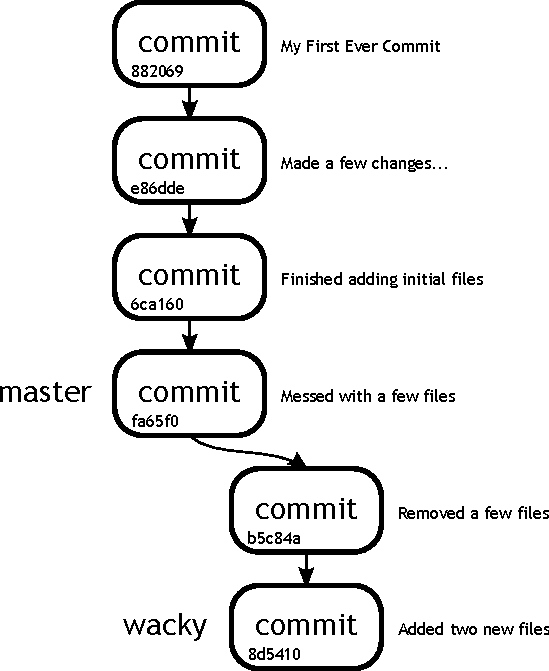
\includegraphics[width=9cm]{images/f-w4-d1.pdf}
\caption{Our first branch}
\end{figure}

So there are really two pointers in our repository at the moment, from a branch point of view.  One of them points to commit \textbf{a022d4d\ldots} and is called \textbf master.  The other is called \textbf{wacky} and points to \textbf{55fb69f
\ldots}.  At this point you may be thinking that branches are pretty much the same thing as tags.  Well, they are except for one important fact.  We are going to use our \texttt{git branch} command, with a new parameter, to show us the difference.  Take a look at the output of the following operations.  We have pruned the output of the \texttt{git show} command for brievity.

\begin{Verbatim}[frame=leftline,framerule=1mm,fontsize=\relsize{-3}] 
john@satsuki:~/coderepo$ git checkout wacky 
Switched to branch 'wacky'
john@satsuki:~/coderepo$ git branch -v
  master a022d4d Messed with a few files
* wacky  55fb69f Added two new files
john@satsuki:~/coderepo$ git tag v2.0
john@satsuki:~/coderepo$ git show v2.0
commit 55fb69f4ad26fdb6b90ac6f43431be40779962dd
...
...
...
\end{Verbatim}

So here we have added a tag in our current branch, \textbf{wacky}, and we can see that the commit ID for the tag \textbf{v2.0} points \textbf{55fb69f}.  We can also see that the branch \textbf{wacky} is currently pointing to the same commit ID, \textbf{55fb69f}.  Now let us add another file in, make a commit and see what happens after this.

\begin{Verbatim}[frame=leftline,framerule=1mm,fontsize=\relsize{-3}] 
john@satsuki:~/coderepo$ echo "New stuff" > another_file
john@satsuki:~/coderepo$ git add another_file
john@satsuki:~/coderepo$ git commit -m 'Added another file'
[wacky 9710177] Added another file
 1 files changed, 1 insertions(+), 0 deletions(-)
 create mode 100644 another_file
john@satsuki:~/coderepo$ git show v2.0
commit 55fb69f4ad26fdb6b90ac6f43431be40779962dd
...
...
...
john@satsuki:~/coderepo$ git branch -v
  master a022d4d Messed with a few files
* wacky  9710177 Added another file
john@satsuki:~/coderepo$ 
\end{Verbatim}

How interesting.  The difference between tags and branches now becomes pretty clear.  Whilst a tag always points to the same commit, a branch reference always points to the tip of that branch.  In essence the reference that a branch points to moves as subsequent commits are made.  By doing this, the whole history of the branch can be retraced.  Since we know the latest commit, we also know the parent of that commit and so on and so on.

Since a branch is just a pointer to a commit, performing operations like adding, modifying and deleting files in the repository can be done safely, without destroying any data in another branch.  In short, it will allow us to completely redesign whatever is being stored in the current branch without worrying about how it will affect our baseline.  For a developer, this is pretty crucial stuff.  This gives people the chance to play with their data and experiment, which is often where the greatest ideas come from.

\section{Day 2 - ``Branches galore''}
\subsection{Working with branches}

Now we know about branches in general, we should really learn about how to merge changes from one branch into another.  Branches are fantastic for trying new things out and testing ideas, but if those ideas are successful, we need a way of pulling those changes into our \textbf{master} branch.  

Of course we could do this the old fashioned way.  We could switch into our \textbf{wacky} branch, do a little development, copy the files somewhere else, switch to our \textbf{master} branch, and paste the files over the top.  Now, this is probably the simplest way of merging possible.  In actual fact, this is not really merging at all.  However one thing that would be lost is the history of how that branch has developed over time.  Sometimes this can be crucial for knowing why certain things were changed during the development process.

Let us take a litle look at the command output of a simple merge, explain it a little, and then look at a diagramatic representation.

\begin{Verbatim}[frame=leftline,framerule=1mm,fontsize=\relsize{-3}] 
john@satsuki:~/coderepo$ git branch
  master
* wacky
john@satsuki:~/coderepo$ 
\end{Verbatim}

Firstly we check just to see what branch we are on.  Next we checkout the branch we want our development branch to be merged into.  In this case, we want to merge \textbf{wacky} into \textbf{master} and so we must first checkout the \textbf{master} branch.  Then we can merge in the changes from our \textbf{wacky} branch.

\begin{Verbatim}[frame=leftline,framerule=1mm,fontsize=\relsize{-3}] 
john@satsuki:~/coderepo$ git checkout master
Switched to branch 'master'
john@satsuki:~/coderepo$ 
\end{Verbatim}

Now we can run the actual merge.

\begin{Verbatim}[frame=leftline,framerule=1mm,fontsize=\relsize{-3}] 
john@satsuki:~/coderepo$ git merge wacky 
Updating a022d4d..9710177
Fast-forward
 another_file             |    1 +
 my_first_committed_file  |    1 -
 my_second_committed_file |    1 -
 newfile1                 |    1 +
 newfile2                 |    1 +
 5 files changed, 3 insertions(+), 2 deletions(-)
 create mode 100644 another_file
 delete mode 100644 my_first_committed_file
 delete mode 100644 my_second_committed_file
 create mode 100644 newfile1
 create mode 100644 newfile2
john@satsuki:~/coderepo$ 
\end{Verbatim} 

We can see that the first line after our command shows us which commit \textbf{master} is the latest common ancestor to both branches and then which commit is the last in our new branch.  In this case we are merging from \textbf{a022d4d} to \textbf{9710177}.  The line below this is even more important.  This type of merge is called a \emph{fast-forward} merge.  We have not made any changes to our \textbf{master} branch since we began developing and subsequently, after finishing our development work, we literally only require fast-forwarding the \textbf{master} branch to the same point in time as our \textbf{wacky} one.  Beneath this text, we see more information about just what is included in the merge.  

We are going to perform a quick check, to see that we are in fact on the master branch and that the latest log message is the one from the point we last left the \textbf{wacky} branch.

\begin{Verbatim}[frame=leftline,framerule=1mm,fontsize=\relsize{-3}] 
john@satsuki:~/coderepo$ git log -n1
commit 9710177657ae00665ca8f8027b17314346a5b1c4
Author: John Haskins <john.haskins@tamagoyakiinc.koala>
Date:   Fri Apr 1 00:16:17 2011 +0100

    Added another file
john@satsuki:~/coderepo$ git branch
* master
  wacky
john@satsuki:~/coderepo$ 
\end{Verbatim}

Now let us take a quick look at a diagram to see how this change actually affected the commit flow.  We have included tags in this diagram, so that you can see where they point to as well.

\begin{figure}[hbt]
\centering
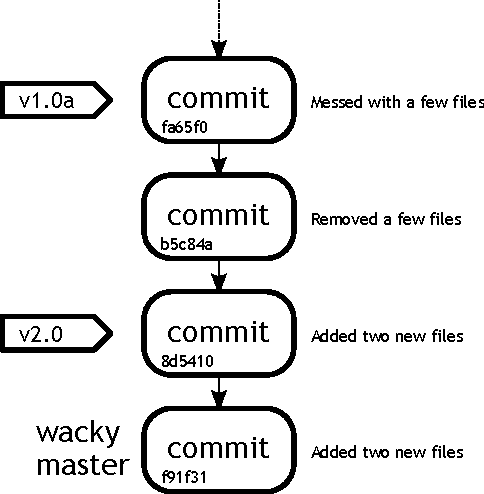
\includegraphics[width=9cm]{images/f-w4-d2.pdf}
\caption{Our first merge}
\end{figure}

This picture should make it clear that the fundamental difference between tags and branches is that whilst the pointer to a branch moves with each commit to that branch, a tag points to a single commit only and never changes, unless forcibly so by the user.

There are a number of tricks that we can employ when using branches.  They are possible because of the super flexible way in which branches are implemented in Git.  As a branch is literally a pointer to a commit, certain operations are available to a user that other systems just can not implement.  However, we should point something out at this point.  Even though we have not yet made any of our repositories public or available to other people, something should always be in the back of your mind.  Allow a few minutes to read the next few paragraphs below.

As someone once said, ``With great power, comes great responsibility.''  Git is hugely powerful.  However, with this power comes a certain level of responsibility.  We are referring here to Git's ability to change history.  If you have watched any science fiction films involving time travel, you should be aware of the difficulties and problems often associated with time travel.  In Git, the same rule applies and the basics of the rule boil down to this: \textbf{If you have made a commit, or path of commits available, you should never ever change anything in the history of those commits or the commits themselves.}  

If you are wondering why this is so important, consider this.  If you are making a series of films, and you have already released the first two of a trilogy, you would not put elements in the third one that contradict the history of the others.  You can not just act like the history of the first two did not happen.  Occasionally this happens in the film industry and what is the reaction of the public?  People get mad.  Sometimes very mad.  This is what will happen if you do the same with Git.  People who are using your repository will end up with many problems and inconsistencies.  \textbf{Do NOT do it, ever}.  There are ways to revert certain behaviour and we will cover this at a later stage.

Having said this, you should not shy away from the awesome capabilities of Git.  We are going to cover a few situations now which you may find yourself in.  Some of them do alter history, some of them do not.  This is why it is important to have an understanding of how Git works.  It can be your best friend, but it can also cause you issues.  If you take the time to tame the beast, it will be one of the most awesome tools in your developers tool bag and can save your life time and time again.  

\begin{trenches}
``Oh man.'' The familiar cry of Simon needing something reverberated round the office.  Rob could never understand why he didn't ask for help.  Simon would sit there wallowing out loud until someone could take it no longer and would eventually go over and help him.

``What to do\ldots what to do.''

Rob could take it no more.  Simon had been exclaiming now for about five minutes and Rob seemed to either be the only one who wasn't listening to music, or who was getting annoyed.  He rolled his eyes, ``What's up Si?''

Simon grinned inanely to himself.  ``I just started modifying some files and well \ldots I don't want to get rid of them \ldots I'm not 100\% sure what I've changed.  I wish I had started this in a new branch.''

``Well, when did you last commit?''

``Just before I started all this work,'' came the reply.

Rob pointed at Simon's screen.  ``You can just create a new branch now and move all the changes into it in one go.  You can do it in one command actually.''
\end{trenches}

It is one hundred percent true.  How many times have you been working on something and wished that you could move all the changes you had made to a new safe environment to protect your already good, working code.  Well, the new safe environment we spoke of sounds suspiciously like a branch.  In Git, any changes you have in your working copy can be taken into a new branch by issuing one command.  It is important to note that these changes can also be taken into an existing branch, but you may run into problems if those changes conflict with items already in that branch.

For now let us see how we can take our working copy changes into a new branch to continue development of some wonderful new feature.  We are going to start by making some changes to our newfiles.

\begin{Verbatim}[frame=leftline,framerule=1mm,fontsize=\relsize{-3}] 
john@satsuki:~/coderepo$ echo "and some more changes" >> newfile1
john@satsuki:~/coderepo$ echo "and a new feature" >> newfile2
john@satsuki:~/coderepo$ 
\end{Verbatim}

Now we are going to make a new branch and switch into it.

\begin{Verbatim}[frame=leftline,framerule=1mm,fontsize=\relsize{-3}] 
john@satsuki:~/coderepo$ git checkout -b wonderful
M	newfile1
M	newfile2
Switched to a new branch 'wonderful'
john@satsuki:~/coderepo$ 
\end{Verbatim}

Did you see that?  We managed to create a new branch and move into it in one go.  The \texttt{git checkout} command is usually what we would use to move into a branch, not create it.  When we use the \texttt{-b} parameter, the \texttt{git checkout} command can be used to create a new branch and switch to it in one go.  Notice we have chosen the name \textbf{wonderful} for this particular branch.  There is also a status output below this that shows we have pulled two modifications into this branch, denoted by the letter \texttt{M} in front of the file name.

Now we can commit these changes.

\begin{Verbatim}[frame=leftline,framerule=1mm,fontsize=\relsize{-3}] 
john@satsuki:~/coderepo$ git commit -a -m 'Fantastic new feature'
[wonderful cfbecab] Fantastic new feature
 2 files changed, 2 insertions(+), 0 deletions(-)
john@satsuki:~/coderepo$ git diff master wonderful 
diff --git a/newfile1 b/newfile1
index 24e7dfa..ef20984 100644
--- a/newfile1
+++ b/newfile1
@@ -1 +1,2 @@
 A new file
+and some more changes
diff --git a/newfile2 b/newfile2
index cba16cc..dac4357 100644
--- a/newfile2
+++ b/newfile2
@@ -1 +1,2 @@
 Another new file
+and a new feature
john@satsuki:~/coderepo$ 
\end{Verbatim}

After running the diff, we can see the differences between the \textbf{master} and the \textbf{wonderful} branches.  Looking more closely at the hunks, the only differences between the two branches are those that we made before we created our \textbf{wonderful} branch.  We have achieved what we set out to in bringing uncommitted changes from \textbf{master} into \textbf{wonderful} and subsequently committing them.

\section{Day 3 - ``Tricking the twigs''}
\subsection{More neat ways to work with branches}

This is only the beginning of the fantastic feature set that Git offers.  By knowing how Git handles your data, you can make it work for you.  Let us take a look at another situation you may find yourself in.

\begin{trenches}
``Rob!'' shouted Simon for the fourth time that morning.  ``Rob, I made a real boo boo this time.''

Rob walked over to Simon again, head lolling back on his shoulders and his eyes rolling.  His arms weighed heavily by his side and his walk reminded Simon of that of a zombie.

``What have you done THIS time?'' asked the developer as he reached the desk.

Simon drew in his breath deeply, ``Well, I created a branch, started working away, committing like a good'un, but I only just realised I'm on the wrong branch.  I forgot to switch.''  He hung his head in shame.  ``I'm screwed right?''

``Not necessarily,'' replied his colleague.
\end{trenches}

This wouldn't work in all situations, but then there are other techniques described later in the book to deal with more special cases.  In this scenario we have created a branch, forgotten to switch into it, and carried on committing as if we were in our new branch.  At first glance it may seem as if we are stuck.  Once we have committed, we can't undo those commits right?  Well, that's not entirely accurate.  

We actually have two ways of clearing up this particular situation.  The first of these is to use \texttt{git revert} to undo the changes of each commit.  Whilst this will work, we have two problems, a) we do not know how to use the \texttt{git revert} tool yet, and b) we can actually handle this situation much more cleanly.  We are going to make a new branch, make a few commits and then look at a diagram of our recent work to see how we can work things out.

\begin{Verbatim}[frame=leftline,framerule=1mm,fontsize=\relsize{-3}] 
john@satsuki:~/coderepo$ git checkout master
Already on 'master'
john@satsuki:~/coderepo$ git branch zaney
john@satsuki:~/coderepo$ echo "and some awesome changes" >> newfile1
john@satsuki:~/coderepo$ git commit -a -m 'Made an awesome change'
[master a27d49e] Made an awesome change
 1 files changed, 1 insertions(+), 0 deletions(-)
john@satsuki:~/coderepo$ echo "and some more awesome changes" >> newfile2
john@satsuki:~/coderepo$ git commit -a -m 'Made another awesome change'
[master 7cc32db] Made another awesome change
 1 files changed, 1 insertions(+), 0 deletions(-)
john@satsuki:~/coderepo$ 
\end{Verbatim}

\begin{figure}[hbt]
\centering
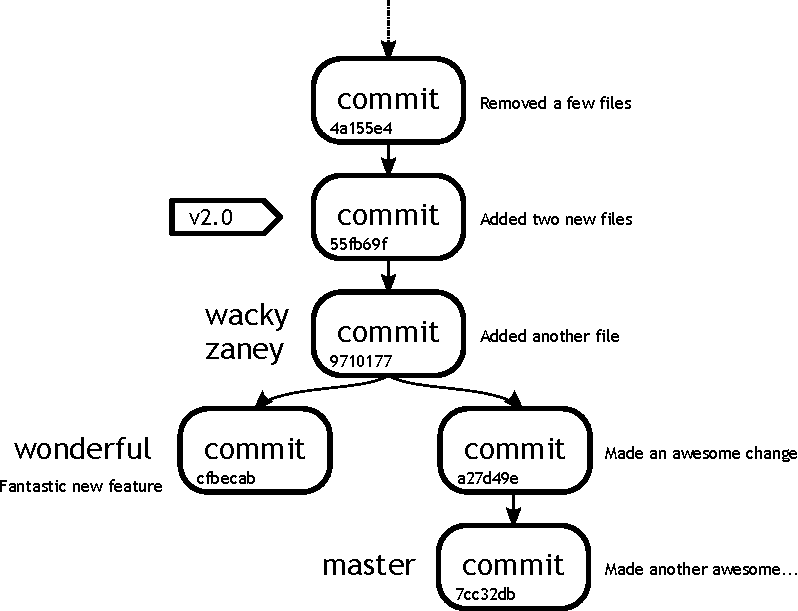
\includegraphics[width=9cm]{images/f-w4-d3.pdf}
\caption{Repository including the mistake}
\end{figure}

\begin{figure}[hbt]
\centering
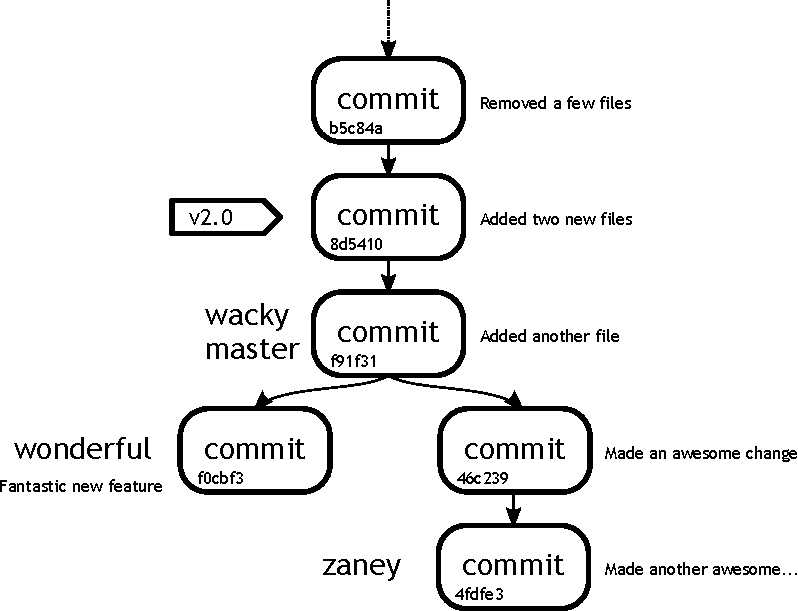
\includegraphics[width=9cm]{images/f-w4-d4.pdf}
\caption{Repository showing how things \emph{should} look}
\end{figure}

Figure 3 shows how our repository looks now, whereas Figure 4 shows how the repository should have looked if we had performed it properly.  You should notice that the positions of \texttt{master} and \texttt{zaney} have switched places.  How can we recify this?

We already discussed one method using \texttt{git revert}, which we are due to cover a little later.  However, because of the way that the history has been written, we can do something very simple.  We are going do the following the following steps.

\begin{enumerate}
\item Switch to our \textbf{zaney} branch
\item Fast-forward our zaney branch so that it points to the same commit using a merge
\item Switch back to our \textbf{master} branch
\item Reset our master branch back to the required point in time
\end{enumerate}

So let us take a look at the command line output and see how we achieve this.  Hopefully you should be familiar with most of the commands.

\begin{Verbatim}[frame=leftline,framerule=1mm,fontsize=\relsize{-3}] 
john@satsuki:~/coderepo$ git checkout zaney
Switched to branch 'zaney'
john@satsuki:~/coderepo$ git merge master
Updating 9710177..7cc32db
Fast-forward
 newfile1 |    1 +
 newfile2 |    1 +
 2 files changed, 2 insertions(+), 0 deletions(-)
john@satsuki:~/coderepo$ git checkout master
Switched to branch 'master'
john@satsuki:~/coderepo$ 
\end{Verbatim}

Now we reach step 4 in our set of instructions.  The one function we do not know how to perform yet is the resetting of our branch back to a previous point in time.  The point we need to rewind back to is the point that we initially created the \textbf{zaney} branch at.  We could have gotten this information by using \texttt{git log}.  Instead, this time we can use the information presented in the merge output to show the common ancestor, which has to be the point that we created our branch at.  In this case it is commit \textbf{9710177}.

We are now going to perform the last step using an old friend called \texttt{git reset}.  You may be thinking that \texttt{git reset} is only used to reset files in the index, but in fact, \texttt{git reset} can actually perform many more tasks.  We are going to use it with the \texttt{--hard} option.  This option can be dangerous, as it will discard all modifications in the working tree, so use with caution.  If we had uncommitted changes in our repository at this point, we could not have used this option.  Let's use the command and see where we get.

\begin{Verbatim}[frame=leftline,framerule=1mm,fontsize=\relsize{-3}] 
john@satsuki:~/coderepo$ git reset --hard 9710177
HEAD is now at 9710177 Added another file
john@satsuki:~/coderepo$ 
\end{Verbatim}

As you can see, we are told that the HEAD of our master branch is now at commit \textbf{9710177}.  We have successfully rewound our \textbf{master} branch to a previous state.  The \texttt{--hard} parameter reset the index and the working tree to be at the state of the commit we tell it to.  It disregards all working copy and staged modifications, so use it with care.

The \texttt{git reset} command does not only work for rewinding back in time.  It can also be used to move a branch forward in time.  As an example of this, we used a fast-forward merge to move our \textbf{zaney} branch forward to be inline with master.  We could just have easily used \texttt{git reset --hard 7cc32db} from within the zaney branch, to bring it to the same point as the master.  In fact, though it looks scary, we could also have used \texttt{git reset --hard master} to reset the \textbf{zaney} branch to be at the same point as \textbf{master}.  Saves typing out those horrid commits does it not?

Finally we are going to introduce one more use of the \texttt{git log} command to show us how our repository looks in a semi-graphical way.

\begin{Verbatim}[frame=leftline,framerule=1mm,fontsize=\relsize{-3}] 
john@satsuki:~/coderepo$ git log --graph --pretty=oneline --all 
--abbrev-commit  --decorate
* 7cc32db (zaney) Made another awesome change
* a27d49e Made an awesome change
| * cfbecab (wonderful) Fantastic new feature
|/  
* 9710177 (HEAD, wacky, master) Added another file
* 55fb69f (v2.0) Added two new files
* 4a155e4 Removed a few files
* a022d4d (tag: v1.0b, v1.0a) Messed with a few files
* 9938a0c Finished adding initial files
* 163f061 (v0.9) Made a few changes to first and second files
* cfe23cb My First Ever Commit
john@satsuki:~/coderepo$ 

\end{Verbatim}

The \texttt{--graph} parameter, tells Git to draw a graph down the left hand column.  The \texttt{--pretty=oneline} parameter reduces the commit details to one line, else we see the entire log message of the commit.  \texttt{--all} shows all branches.  The \texttt{abbrev-commit} in the command tells Git to abbreviate the commit IDs to a sensible length.  Finally, \texttt{--decorate} shows us the tag and branch references.  Hopefully if you compare this tree to the diagram earlier, you will see that the tree is actually completely in order.

Be aware that during this work we have changed the history of at least one of our branches.  Had we pushed our changes to a public server, which is something that will be discussed next week, we would have to force these changes to be accepted at the server end.  Git knows we are trying to change a past that may have been viewed by others and will warn us accordingly.

\section{Day 4 - ``I pressed delete...''}
\subsection{Handling the pressure}

We have had some awesome fun working with branches, and hopefully you can see how utterly powerful Git is.  Sometimes though we can get ourselves into trouble and it is here that Git can also come to our rescue.  Let us learn how to delete a branch.  We are going to delete our \textbf{wacky} branch now as we have already merged it and no longer require it.

\begin{Verbatim}[frame=leftline,framerule=1mm,fontsize=\relsize{-3}] 
john@satsuki:~/coderepo$ git branch -d zaney 
error: The branch 'zaney' is not fully merged.
If you are sure you want to delete it, run 'git branch -D zaney'.
john@satsuki:~/coderepo$ git branch -D zaney
Deleted branch zaney (was 7cc32db).
john@satsuki:~/coderepo$ git branch -v
* master    9710177 Added another file
  wacky     9710177 Added another file
  wonderful cfbecab Fantastic new feature
john@satsuki:~/coderepo$ 
\end{Verbatim}

Ooops.  Despite the firm warning from Git, we have inadvertantly deleted the \textbf{zaney} branch by mistake.  This does happen.  When people are in the thick of it, they do make mistakes and it is comforting to know that Git is able to recover from this, but how?  We have deleted the branch reference that pointed to the commit that was at the tip of the \textbf{zaney} branch by using the \texttt{-d} and \texttt{-D} parameters.  So the question is, does that commit still exist any more?  Maybe we did more damage than we thought.  By deleting all references to the commit, how do we get it back?

All is most definitely not lost.  Even though we have removed all references to the commits in question, they still exist in the repository.  They will continue to so unless we run a clean up on the repository, which will be covered later, or if the items are left to age for more that at least fourteen days.  This means that we have up to two weeks to try to recover the lost commits.  Of course in practice one would hope that we would perform the recovery much earlier than that.

We already know the commit ID that the branch was pointing to.  Git has been very kind and told us it, just before it carried out the delete.  We are looking for commit \textbf{7cc32db}.  If we run the command below, we will create and recover our branch in one go.

\begin{Verbatim}[frame=leftline,framerule=1mm,fontsize=\relsize{-3}] 
john@satsuki:~/coderepo$ git branch zaney 7cc32db
john@satsuki:~/coderepo$ git branch -v
* master    9710177 Added another file
  wacky     9710177 Added another file
  wonderful cfbecab Fantastic new feature
  zaney     7cc32db Made another awesome change
john@satsuki:~/coderepo$ 
\end{Verbatim}

Our branch has been restored and points to the same place as it did before we deleted it.  As each commit points to its parent, we now have the complete history of \textbf{zaney} restored and the branch can be used as normal.  To complete this action, let us delete the \textbf{wacky} branch as originally intended.

\begin{Verbatim}[frame=leftline,framerule=1mm,fontsize=\relsize{-3}] 
john@satsuki:~/coderepo$ git branch -d wacky
Deleted branch wacky (was 9710177).
john@satsuki:~/coderepo$ git branch -v
* master    9710177 Added another file
  wonderful cfbecab Fantastic new feature
  zaney     7cc32db Made another awesome change
john@satsuki:~/coderepo$ 
\end{Verbatim}

As you can see, when we deleted \textbf{wacky} we were not warned about unmerged changes.  This is because the \textbf{wacky} branch is at the same point as the \textbf{master} branch.  

\section{Day 5 - ``Conflicting information''}
\subsection{What to do when it all goes wrong}

The team have been playing with branches for a few days now and are beginning to settle into the idea of branching often.  As you can see, in Git, a branch is a really simple device for allowing experimentation and development.  As the implementation of branches is so simple, it is also really fast to switch between branches.  If you have been keeping up with the \emph{After Hours} sections, you can hopefully see that when switching branches, Git only needs to alter what is different between one working copy and another.

Let us see what new issues the team runs into during Week 4.

\begin{trenches}
``Hmm,'' the puzzled noise reverberated round Klaus' corner of the office.  Mumbling commenced.  ``So if I did that, then why is that not \ldots I mean I didn't think \ldots that's probably the problem Klaus \ldots sill 'luser'.''  He chuckled to himself, hardly noticing the looming figure of John.

``You got a conflict,'' said John matter of factly.

``I can see that,'' came Klaus' reply.  ``The problem is how do I solve it''

``What were you doing?''

``Well I had a few branches I had been working on and I was trying to merge them in.''

``Figures,'' said John.  
\end{trenches}

Conflicts are bound to happen at some point.  Even the best project processes in the world will sometimes end up with a conflict that has to be resolved.  We should, at this point, clarify what a conflict actually is.  A conflict occurs when an attempt is made to reconcile multiple changes to the same section of a file at the same time.  This usually means that the same line of code is modified by two different parties at the same time.  Now that we have several branches in our test repository, let us merge them back into master and see if we come up with a conflict.

First we are going to add a little change to one of our files.

\begin{Verbatim}[frame=leftline,framerule=1mm,fontsize=\relsize{-3}] 
john@satsuki:~/coderepo$ echo "Another update to this file" >> my_third_committed_file 
john@satsuki:~/coderepo$ git commit -a -m 'Updated third file'
[master 4ac9201] Updated third file
 1 files changed, 1 insertions(+), 0 deletions(-)
john@satsuki:~/coderepo$ 
\end{Verbatim}

Now let us merge in our \textbf{wonderful} branch.

\begin{Verbatim}[frame=leftline,framerule=1mm,fontsize=\relsize{-3}] 
john@satsuki:~/coderepo$ git merge wonderful
Merge made by recursive.
 newfile1 |    1 +
 newfile2 |    1 +
 2 files changed, 2 insertions(+), 0 deletions(-)
john@satsuki:~/coderepo$ 
\end{Verbatim}

So far, our merge has gone pretty well.  We have taken all of the changes that were made in the \textbf{wonderful} branch and pulled them into our \textbf{master} branch.  If we wanted to, we could continue on making changes to the \textbf{wonderful} branch and we could keep pulling changes in from one to the other as time went by.  Figure 5 shows what our repository looks like now.

\begin{figure}[hbt]
\centering
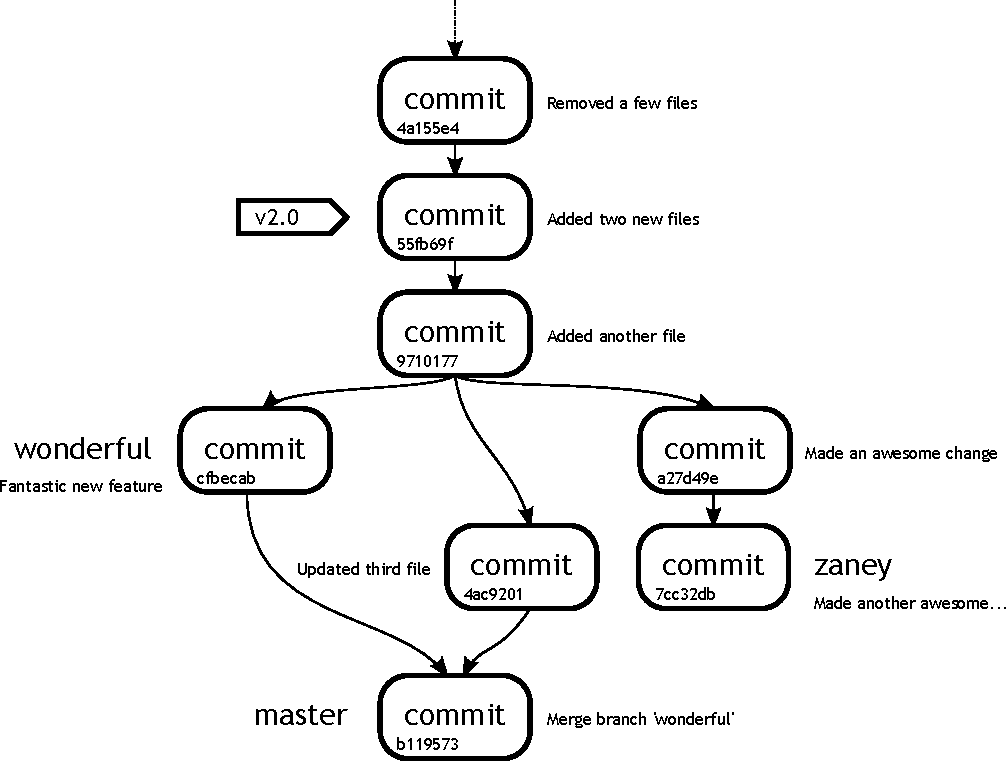
\includegraphics[width=9cm]{images/f-w4-d5.pdf}
\caption{Repository state after \textbf{wonderful} merge}
\end{figure}

Our repository tree looks a little strange now.  Notice that the most recent commit, \textbf{b119573}, has two parents.  Can this be true?  If we run our \texttt{git show} command against that commit ID, we see something new.

\begin{Verbatim}[frame=leftline,framerule=1mm,fontsize=\relsize{-3}] 
john@satsuki:~/coderepo$ git show b119573
commit b119573f4508514c55e1c4e3bebec0ab3667d071
Merge: 4ac9201 cfbecab
Author: John Haskins <john.haskins@tamagoyakiinc.koala>
Date:   Fri Apr 1 07:35:13 2011 +0100

    Merge branch 'wonderful'

john@satsuki:~/coderepo$ 
\end{Verbatim}

Notice the line \texttt{Merge: 4ac9201 cfbecab}, which simply tells us that this is a special type of commit, a merge commit.  When we previously performed a merge, the branch we were merging back into had not changed since we branched off and did our development work.  If you remember, we called this a \emph{fast-forward} merge, simply because we moved our \emph{destination} branch forwards to meet the tip of the development branch.

This time things are a little different.  During out development time on \textbf{wonderful}, something changed on \textbf{master}.  We did not make many alterations, but just the fact that we made some changed the way the merge was performed.  In fact, we can see this if we look at the first line after the merge.  Instead of indicating a \emph{fast-forward} merge, it now states that the merge was \emph{recursive}.  If you are interested in the different types of merge algorithms, you should read the \emph{After Hours} section for this chapter.

So now the history of this latest commit actually relies on two previous commits.  The changes that have been introduced in these commits are merged together to form a combined tree of files.  This is the snapshot that is represented in commit \textbf{ba0bfc}.

Let us now remove that third file before merging in the \textbf{zaney} branch.

\begin{Verbatim}[frame=leftline,framerule=1mm,fontsize=\relsize{-3}] 
john@satsuki:~/coderepo$ git rm my_third_committed_file
rm 'my_third_committed_file'
john@satsuki:~/coderepo$ git commit -a -m 'Removed third file'
[master ed2301b] Removed third file
 1 files changed, 0 insertions(+), 2 deletions(-)
 delete mode 100644 my_third_committed_file
john@satsuki:~/coderepo$ 
\end{Verbatim}

So now we are ready to merge in the \textbf{zaney} branch.

\begin{Verbatim}[frame=leftline,framerule=1mm,fontsize=\relsize{-3}] 
john@satsuki:~/coderepo$ git merge zaney
Auto-merging newfile1
CONFLICT (content): Merge conflict in newfile1
Auto-merging newfile2
CONFLICT (content): Merge conflict in newfile2
Automatic merge failed; fix conflicts and then commit the result.
john@satsuki:~/coderepo$ 
\end{Verbatim}

Oh dear!  That probably did not go as well as we had hoped.  We have two conflicts.  The first is in \texttt{newfile1} and the second in \texttt{newfile2}.  You may be wondering why.  The last commit we made did not make any changes to either of those files, so why do we suddenly have a conflict?  When using a version control system like Git, conflicts are an every day part of life.  A conflict does not mean you have done something wrong.  It simply means that the automatic merging algorithm can not merge the changes.

In this case we have a conflict because the files have changed in both sides of the merge, since they diverged.  Rephrasing this slightly: Since the point when we created the branch \textbf{zaney}, at commit \textbf{55fb69}, both the \textbf{master} branch and the \textbf{zaney} branch have both modified the same files in the same places.  Right now, our merge is paused.  For now, let us abort the merge so that we can take a closer look at what happened.

\begin{Verbatim}[frame=leftline,framerule=1mm,fontsize=\relsize{-3}] 
john@satsuki:~/coderepo$ git reset --merge
john@satsuki:~/coderepo$ 
\end{Verbatim}

So let us compare the changes between our latest common ancestor and our branch tips.  We will first look at the difference between the ancestor and our \textbf{master} branch, but limit it to the files with conflicts.

\begin{Verbatim}[frame=leftline,framerule=1mm,fontsize=\relsize{-3}] 
john@satsuki:~/coderepo$ git diff 55fb69 master -- newfile*
diff --git a/newfile1 b/newfile1
index 24e7dfa..ef20984 100644
--- a/newfile1
+++ b/newfile1
@@ -1 +1,2 @@
 A new file
+and some more changes
diff --git a/newfile2 b/newfile2
index cba16cc..dac4357 100644
--- a/newfile2
+++ b/newfile2
@@ -1 +1,2 @@
 Another new file
+and a new feature
john@satsuki:~/coderepo$ 
\end{Verbatim}

Now we will do the same between the common ancestor and the tip of \textbf{zaney}.

\begin{Verbatim}[frame=leftline,framerule=1mm,fontsize=\relsize{-3}] 
john@satsuki:~/coderepo$ git diff 55fb69 zaney -- newfile*
diff --git a/newfile1 b/newfile1
index 24e7dfa..d94dacc 100644
--- a/newfile1
+++ b/newfile1
@@ -1 +1,2 @@
 A new file
+and some awesome changes
diff --git a/newfile2 b/newfile2
index cba16cc..45659d7 100644
--- a/newfile2
+++ b/newfile2
@@ -1 +1,2 @@
 Another new file
+and some more awesome changes
john@satsuki:~/coderepo$ 
\end{Verbatim}

So hopefully you can see that we have tried to change the second line in both files.  This is where the conflict is arising from.  Let us try to run the merge again and this time we will resolve the conflicts manually.

\begin{Verbatim}[frame=leftline,framerule=1mm,fontsize=\relsize{-3}] 
john@satsuki:~/coderepo$ git merge zaney
Auto-merging newfile1
CONFLICT (content): Merge conflict in newfile1
Auto-merging newfile2
CONFLICT (content): Merge conflict in newfile2
Automatic merge failed; fix conflicts and then commit the result.
john@satsuki:~/coderepo$ cat newfile1
A new file
<<<<<<< HEAD
and some more changes
=======
and some awesome changes
>>>>>>> zaney
john@satsuki:~/coderepo$ cat newfile2
Another new file
<<<<<<< HEAD
and a new feature
=======
and some more awesome changes
>>>>>>> zaney
john@satsuki:~/coderepo$ 
\end{Verbatim}

We have displayed the contents of \texttt{newfile1} and \texttt{newfile2} during this merge.  At the moment, no commits have been made and we have a chance to tell Git exactly what these files should look like.  You should be able to see that Git has modified the files to show us what both the branches think the file should look like.  At the top, just after the \texttt{<<<<<<< HEAD} is how the line was modified in the \textbf{master} branch.  We then have a divider \texttt{=======} and after that we have the line, as it was modified in the \textbf{zaney} branch, followed by \texttt{>>>>>>> zaney}.  We can now edit these files manually, remove the dividers, header and footer and commit the result.  

We are going to edit \texttt{newfile1} to look like this:

\begin{Verbatim}[frame=leftline,framerule=1mm,fontsize=\relsize{-3}] 
A new file
and some more awesome changes
\end{Verbatim}

We will also edit \texttt{newfile2} to look like this:

\begin{Verbatim}[frame=leftline,framerule=1mm,fontsize=\relsize{-3}] 
Another new file
and a new awesome feature
\end{Verbatim}

Now we have resolved the conflicts and set the files straight, we can add the files and commit the result.

\begin{Verbatim}[frame=leftline,framerule=1mm,fontsize=\relsize{-3}] 
john@satsuki:~/coderepo$ git add newfile*
john@satsuki:~/coderepo$ git commit -a -m 'Merged in zaney'
[master d50ffb2] Merged in zaney
john@satsuki:~/coderepo$ git log -n2
commit d50ffb2fa536d869f2c4e89e8d6a48e0a29c5cc1
Merge: ed2301b 7cc32db
Author: John Haskins <john.haskins@tamagoyakiinc.koala>
Date:   Fri Apr 1 07:42:04 2011 +0100

    Merged in zaney

commit ed2301ba223a63a5a930b536a043444e019460a7
Author: John Haskins <john.haskins@tamagoyakiinc.koala>
Date:   Fri Apr 1 07:37:34 2011 +0100

    Removed third file
john@satsuki:~/coderepo$ 
\end{Verbatim}

Our merge has been completed.  Let us now see what our repository looks like graphically, in Figure 6.

\begin{figure}[hbt]
\centering
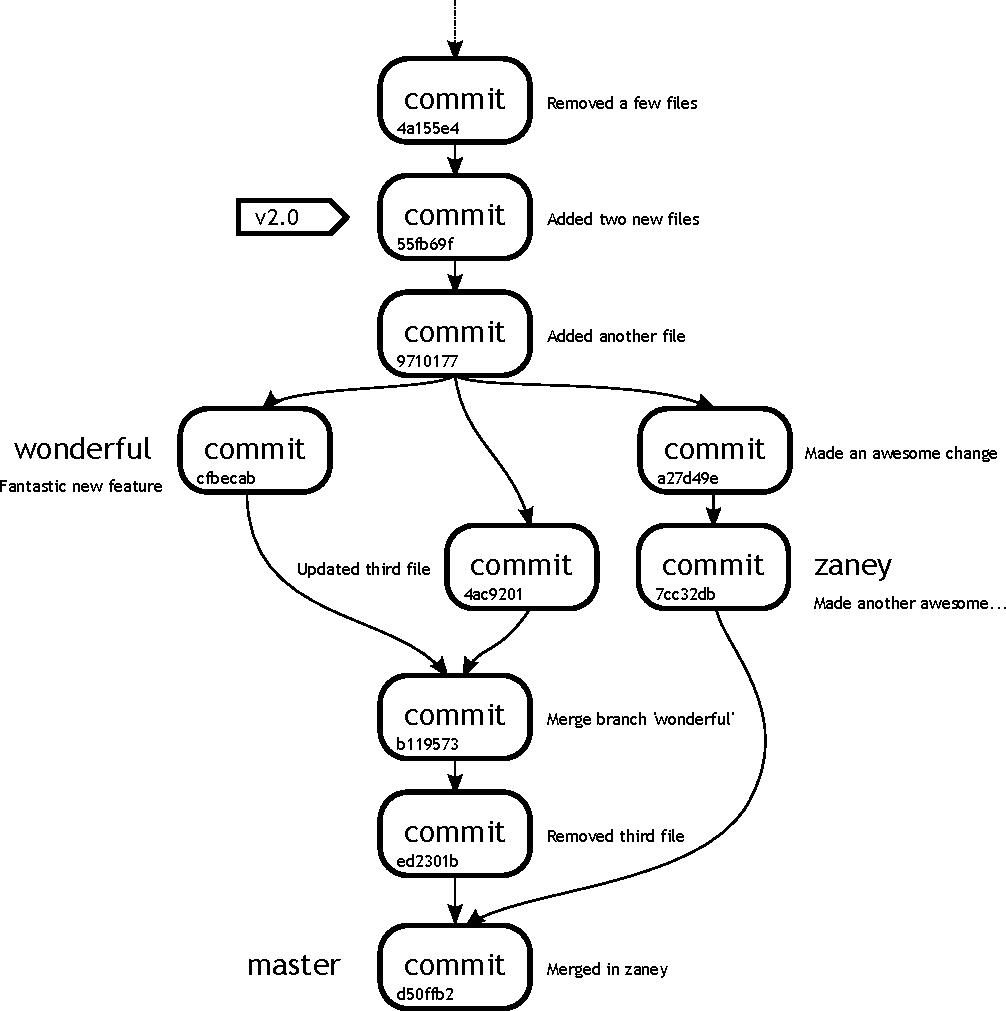
\includegraphics[width=9cm]{images/f-w4-d6.pdf}
\caption{Repository state after \textbf{zaney} merge}
\end{figure}

It is quite reasonable that you may want to continue working on branches after you have integrate those changes back into your master.  Obviously you would have to merge your \textbf{master} branch back into \textbf{zaney} or any of the others, otherwise you could be developing on older versions of the code.  This brings up an interesting point which will be covered in a later chapter, as there are multiple ways to keep a development branch up to date.

So, at the end of this week, we have learnt how to create branches, how to merge them, and how to resolve conflicts.  It should be stressed that a conflict is not a \textbf{bad} thing.  Conflicts do happen and when they do you should simply take your time and resolve the conflict in order to represent the \emph{best of both worlds}.  The \emph{After Hours} section for Week 4, takes a closer look at merging and explains some more about what branches are at a repository level.

\clearpage

\section{Summary - John's Notes}
\subsection{Commands}
\begin{itemize}
\item\texttt{git branch <branch\_name>} - Creates a new branch with a given name

\item\texttt{git checkout <branch\_name>} - Switches to a new branch

\item\texttt{git log -n1} - Limits the output of the log command to only a single commit

\item\texttt{git branch -v} - Verbosely list all local branchs

\item\texttt{git show <reference>} - Show the information pointed to by the reference

\item\texttt{git merge <branch\_name>} - Merge in a given branch to the current one

\item\texttt{git checkout -b <branch\_name>} - Create a new branch and switch into it in one go

\item\texttt{git reset --hard <commit\_ref>} - Reset a branch to a specific commit reference

\item\texttt{git log --graph --pretty=oneline --all --abbrev-commit --decorate} - Shows a graphical view of the repository

\item\texttt{git log --graph --oneline --all --decorate} - A shorter form of the above command

\item\texttt{git branch -d <branch\_name>} - Delete a branch that has already been merged

\item\texttt{git branch -D <branch\_name>} - Forcibly delete a branch

\item\texttt{git branch <branch\_name> <commit\_ref>} - Create a new branch, starting at the commit reference

\item\texttt{git reset --merge} - Abort a merge and reset back to pre-merge state

\item\texttt{git diff <commit\_1> <commit\_2> -- <files>}- Show the difference between the two commits, for certain files

\end{itemize}

\subsection{Terminology}
\begin{itemize}

\item\textbf{Conflict} - A conflict occurs when an attempt is made to reconcile multiple changes to the same section of a file at the same time.

\item\textbf{Fast-forward Merge} - The simplest merge type, which simply winds a branch forward in time to meet the tip of another.

\end{itemize}
